\documentclass[12pt]{article}  % standard LaTeX, 12 point type

\usepackage{geometry}

\usepackage{amsmath}
\usepackage{amsfonts,latexsym}
\usepackage{amsthm}
\usepackage{amssymb}
\usepackage[utf8]{inputenc} % Кодировка
\usepackage[english,russian]{babel} % Многоязычность
\usepackage{verbatim}
\usepackage{longtable}
%\usepackage{lscape}
\usepackage{csvsimple}
\usepackage[toc,page]{appendix}
\usepackage{booktabs}

\usepackage{float}
\usepackage{array}
\usepackage{multirow}
\usepackage{caption}
\usepackage{graphicx}
\usepackage{ucs}
\usepackage{rotating}
\usepackage{pdflscape}
\usepackage{afterpage}
\usepackage{capt-of}% or use the larger `caption` package

% unnumbered environments:

\theoremstyle{remark}
\newtheorem*{remark}{Remark}
\newtheorem*{notation}{Notation}
\newtheorem*{note}{Note}

\setlength{\parskip}{5pt plus 2pt minus 1pt}
\newcolumntype{C}{>{\centering\arraybackslash}p{1.3cm}}
\renewcommand\appendixpagename{Приложение}
\graphicspath{{pics/}}

\title{Использование КС-грамматики для распознавания \\ 16s рРНК}
\author{Semyon Grigorev, Dmitry Kovalev}
\date{\today}

\begin{document}

\newgeometry{left=0.8in,right=0.8in,top=1in,bottom=1in}

\maketitle 

\section{Введение}

Задача поиска и классификации цепочек --- важна.
Некоторые из них используются как маркерные для обнаружения и классификации организмов.
Одна из таких последовательностей --- 16s rRNA.

Вторичная структура достаточно богата.
Более того, известно, что некоторые участки обладают достаточно консервативной вторичной структурой.
Ещё Эдди и коллеги стали использовать информацию о вторичной структуре для классификации.


Грамматика позволяет минимизировать знания о первичной структуре.
Поиск структурного шаблона.
Грамматика задаётся вручную, но возможен и вывод грамматики, но это тема для отдельного исследования.

Данный отчёт описыывает эксперимент по распознованию 16s только на основе вторичной структуры, 
описанной контекстно-свободной граммтикой.

\section{Грамматика}

Используемая грамматика приведена в приложении \ref{grammar}.
Язык описания --- YARD.
В правых частях можно использовать конструкции регулярных выражений.
Четыре терминальных символа-нуклеотида: $A, U, C, G$.
\begin{table}[h]
    \centering
    \renewcommand{\arraystretch}{1.5}
    \begin{tabular}{|c|>{\centering}p{9cm}|}
        \hline
        Грамматическая конструкция & Описание 
        \tabularnewline \hline
        $ any $ & Один из нуклеотидов 
        \tabularnewline \hline
        $ any^*[n..m] $ & Цепочка нуклеотидов длины от $n$ до $m$ 
        \tabularnewline \hline
        $stemN{<}s{>}$  & Стем высоты $N$ со свободной частью $s$ (последовательность любых конструкций грамматики) 
        \tabularnewline \hline
        $mk\_stem{<}s{>}$ & Стем произвольной высоты (от $0$ до $N$) со свободной частью $s$
        \tabularnewline \hline
    \end{tabular}
    \caption{Базовые конструкции грамматики}
\end{table}

\begin{table}[h]
    \centering
    \renewcommand{\arraystretch}{2}
    \begin{tabular}{c | c}
        $stem4{<}any^*[3..5]{>}$ & $mk\_stem{<} any^*[1..2] \ stem2{<} any^*[3..4] {>} \ any^*[2..5] {>}$ \\
        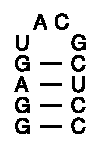
\includegraphics[width=1.5cm]{stem4.pdf} & 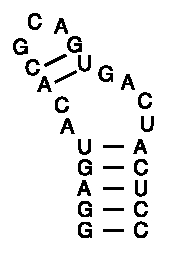
\includegraphics[width=2cm]{mk_stem.pdf} \\
    \end{tabular}
    \caption{Примеры описания структур}
\end{table}

\section{Эксперименты}

Два эксперимента: обработка баз известных 16s, обработка полноразмерных геномов.

\begin{table}[h]
    \centering
    \begin{tabular}{c >{\centering}p{3cm} *{6}{C}}
        \toprule
        \multirow{2}{*}{Домен} & \multirow{2}{*}{\parbox{3cm}{\centering Стартовый нетерминал}} & \multicolumn{2}{c}{Бактерии} & \multicolumn{2}{c}{Эукариоты} & \multicolumn{2}{c}{Археи} \\
        \cmidrule(lr){3-4}
        \cmidrule(lr){5-6}
        \cmidrule(lr){7-8}
        & & Р & НР & Р & НР & Р & НР \\
        \midrule
        Центральный & h19 & 17878 & 335 & 2153 & 3165 & 306 & 13 \\
        5'M & h3 & 11498 & 6715 & 64 & 5254 & 81 & 238\\
        \bottomrule
    \end{tabular}
    \caption{Результаты анализа базы организмов}
\end{table}

Базы размеченных полноразмерных геномов с информацией о 16s: оценить точность, полноту и т.д. (сколько из отмеченных найдено, сколько из отмеченных не найдено, сколько найдено неотмеченных).
Проанализировать ложные срабатывания и пропущенных кандидатов.

\afterpage{
\begin{landscape}
\csvloop{
    file=final_report_middle.csv,
    no head,              % no special treatment of first line
    column count=7,       % since no first line is given, tell about column count
    respect all,
    before reading=
        \begin{table}[p]\centering\footnotesize
        \begin{tabular}{llccccc}\toprule,
    command=\csvlinetotablerow,
    late after line=\\,
    late after first line=\\\midrule,
    late after last line=\\\bottomrule,
    after reading=
        \end{tabular}
        \caption{Результаты анализа полноразмерных геномов (центральный домен)}
        \end{table}
}
\end{landscape}
}

\afterpage{
    \begin{landscape}
        \csvloop{
            file=final_report_head.csv,
            no head,              % no special treatment of first line
            column count=7,       % since no first line is given, tell about column count
            respect all,
            before reading=
            \begin{table}[p]\centering\footnotesize
                \begin{tabular}{llccccc}\toprule,
                    command=\csvlinetotablerow,
                    late after line=\\,
                    late after first line=\\\midrule,
                    late after last line=\\\bottomrule,
                    after reading=
                \end{tabular}
                \caption{Результаты анализа полноразмерных геномов (5'M домен)}
            \end{table}
        }
    \end{landscape}
}

\pagebreak  

\begin{appendices}
\section{Грамматика 16S на языке YARD, использовавшаяся в эксперименте}
\label{grammar}
\verbatiminput{16S_grammar.yrd}
\end{appendices}
\end{document}